\section{Our Implementation}
Having defined an algorithm in Section~\ref{sec:tnfa}, we wished to construct a simple program based on TNFA, which would pattern-match data allowing for mismatches.

% Torbens noter kræver begrundelse for beslutninger, hvorfor bruger vi C++
We wrote a simple program in C++, in order to ensure strict control of the types and behavior of our code. We named the program TNFA Pattern-Matcher (TPaMa). TPaMa is able to create an NFA from a RE, as described in Section~\ref{RA_TO_NFA}, by supporting a series of RE symbols along with concatenation of characters.
% An example of a TFNA from a RE could be RE "(GAT)+" which would produce a structure as shown in Figure~\ref{fig:gat}

%\begin{figure}[h!]
%\centering
%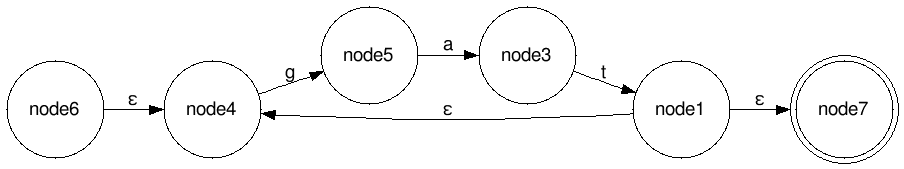
\includegraphics[width=0.5\textwidth]{lib/gat.png}
%\caption{Example of how TPaMa constructs a TNFA from RE (GAT)+}
%\label{fig:gat}
%\end{figure}

Currently the search implementation of TPaMa only support simple patterns such as "GAT", which does not cause any $\epsilon$-transitions to be constructed. This choice was made, so we could focus on the performance of mismatching while giving support to the most crucial part of pattern-matching.

This also meant that determining reachable states, as mentioned in Algorithm~\ref{tnfasim} \&~\ref{tnfatrans}, is rather straightforward, as there's only up to one possible next state for every state (zero for the final state). 

To handle mismatching, recall Table~\ref{nfac}:

%\begin{table}[h]
\begin{tabular}{*{2}{m{0.4\textwidth}}}
\begin{center}$a$\end{center} &\begin{center}
\begin{tikzpicture}[->,>=stealth,shorten >=1pt,auto,node distance=2 cm, scale = 0.75, transform shape,initial text={}]
  \node [initial, state] (0) {};
  \node [accepting,state, right of=0] (1) {};

  \path[->] (0) edge node [above] {$a$} (1);
  \path[->] (0) edge [color=green, in=100,out=80,loop] node [color=black, above] {$\epsilon/i$} (0);
  \path[->] (0) edge [color=red,bend left] node [color=black, above] {$\epsilon/d$} (1);

  \path[->] (0) edge [color=blue,bend right] node [color=black, below] {$\epsilon/a$} (1);
\end{tikzpicture}\end{center}\\
\end{tabular}
%\end{table}

There's three different types of mismatches. Instead of having three types of transitions, as the theory call for, in the simulation we solve this by having three counters in each state, one for each type of mismatch (insertions, alternation and deletion), keeping track of the remaining number of mismatches allowed in the match. Whenever a match can not be made, for each mismatch counter with a positive value, a new state is created corresponding to the transitions above; alternations and deletions both advance the state to the next reachable, while insertions remain in the same state in the TNFA, the corresponding mismatch counter is decreased and the pattern-matching continues.

For every state in the stateset, at some point it will either match the final state of the TFNA at which point a match is printed, or a state will not be able to match, even with mismatches, at which point it will be erased from the stateset. This continues until all data has been checked, at which point the TPaMa terminates.